\documentclass{brandeis-thesis3.2}
\usepackage[utf8]{inputenc}

\usepackage{hyperref}
\usepackage[round]{natbib}

\renewcommand{\bibsection}{\chapter*{References}\addcontentsline{toc}{chapter}{References}
}
\setcounter{secnumdepth}{5}
\usepackage{romannum}
\usepackage{amssymb}
\usepackage{amsmath}
\usepackage{wasysym}
\usepackage{tabularx} % extra features for tabular environment
\usepackage{graphicx} % takes care of graphic including machinery
\usepackage{subcaption} % from Jason: subfigures

% short cuts
\def \msun {M_{\odot}}
\newcommand{\iso}[2]{$^{#1}${#2}}
\newcommand{\del}[3]{\delta^{#1}\text{#3}_{#2}}

\bibliographystyle{aasjournal}
\title{The Impact of Nuclear Uncertainties on the Galactic Chemical Evolution of Silicon Isotopes in Comparison with Stardust Grains}
\author{Hung Kwan Fok}

\graduationmonth{May}
\graduationyear{2023}

\program{
  Undergraduate Program in Physics \\
  Department of Physics
}

\degreetype{Science}


\begin{document}

\maketitlepage
\makecopyright

\thispagestyle{empty}
\begin{center}
\vspace*{1cm}
    
    This Senior Honors thesis, directed and approved by Hung Kwan Fok' Committee, has been accepted and\\
    approved by
        
    \vspace{0.75cm}
    the Department of Physics at Brandeis University
        
    \vspace{0.75cm}
    in partial fulfillment of the requirements for the degree of: Bachelor of Science in Physics
    
    \vspace{2cm}
    \noindent\rule{14cm}{0.4pt}\\
    , Undergraduate Advising Head
    
    \vspace{2cm}
    
    Dissertation Committee:\\
    Dr. Reto Trappitsch, Dr. James Cho
    
    \vspace{2cm}
    
    


    \noindent\begin{tabular}{ll}
    \makebox[3in]{\hrulefill} & \makebox[3in]{\hrulefill}\\
    Printed Name & Signature\\[8ex]% adds space between the 2 sets of signatures
    \makebox[3in]{\hrulefill} & \makebox[3in]{\hrulefill}\\
    Printed Name & Signature\\
    \end{tabular}
\end{center}

%\chapter*{Acknowledgments}
%\addcontentsline{toc}{chapter}{Acknowledgments}

% Contain the double spacing in an environment so it doesn't affect the abstract
\begin{doublespacing}


\end{doublespacing}

% Page must be manually cleared before and after abstract since it's not a section/chapter as-is
\clearpage

\begin{thesis-abstract}
\addcontentsline{toc}{chapter}{Abstract}
\textbf{(THIS NEEDS TO BE EDITED)}The major group of presolar SiC grains, the so-called mainstream grains, are believed to have condensed in the outflows of low-mass stars (up to a few solar masses) when they went through the asymptotic giant branch (AGB) phase at the end of their lives. However, the silicon isotopic ratios measured in these grains cannot be explained in terms of the nucleosynthesis in AGB stars. Thus, the grains are believed to carry the signature of galactic chemical evolution (GCE). In particular, the silicon analyzed in mainstream SiC grain represents overall nucleosynthesis in massive stars over roughly 9\,Ga of GCE. Measurements of silicon isotope ratios in mainstream SiC grains suggests that there is a linear correlation between \iso{29}{Si}/\iso{28}{Si} and \iso{30}{Si}/\iso{28}{Si}. However, current GCE models have so far failed to explain the slope of that correlation line. This study aims to investigate how nuclear uncertainties affect the GCE of silicon isotopes, specifically their ratios. First, the impact of nuclear uncertainties on the production of silicon isotopes in the main silicon production zone in massive stars is investigated using the NuGrid nucleosynthesis post processing network (PPN) by varying the relevant reaction rates. Based on the modified yields in the relevant zones, integrated stellar yields will be determined. The silicon isotopic ratios \iso{29}{Si}/\iso{28}{Si} and \iso{30}{Si}/\iso{28}{Si} are then calculated using the detailed NuPyCEE GCE model with the stellar yields modified. These GCE calculations for silicon are then compared with stardust grain measurements. This study will allow us to determine whether the correlation of the silicon isotopes measured in presolar mainstream grains can be explained by nuclear  uncertainties and GCE.

\end{thesis-abstract}

% Page must be manually cleared before and after abstract since it's not a section/chapter as-is
\clearpage

\tableofcontents
\clearpage

% \listoftables
% \addcontentsline{toc}{chapter}{List of Tables}
% \clearpage

% \listoffigures
% \addcontentsline{toc}{chapter}{List of Figures}
% \clearpage

\startbody

\chapter{Introduction}

\section{Galactic Chemical Evolution}

Galactic Chemical Evolution (GCE) refers to the evolution of elements and isotopes in the galaxy. In this section, we will discuss the basic ingredients of GCE models and the different types of models used for GCE.

\subsection{Basic Ingredients}

There are four necessary ingredients for a typical GCE model: initial conditions, the stellar birthrate function, the nucleosynthesis yields recycled back into the galaxy, and the gas inflow and outflow from the galaxy. The chemical abundance of an element $X_i$ over time is generally given by:

\begin{equation}
X_i = \frac{M_i}{M_{\rm gas}}
\end{equation}

where $M_i$ is the mass of the element in the interstellar medium (ISM), and $M_{\rm gas}$ is the total amount of gas.

\subsubsection{Initial Conditions}

The initial conditions of a GCE model refer to the initial composition of the galaxy. One typical initial composition is the primordial abundance, which includes the elements formed in the Big Bang. The initial composition of a GCE model can also be a metal-enriched chemical composition, known as prompt initial enrichment (PIE), which is enriched by an initial generation of Population \Romannum{3} stars. Population \Romannum{3} stars are hypothesized to have no metals.

\subsubsection{Stellar Birthrate Function}

The stellar birthrate function describes the star formation history in a galaxy, and can be written as:

\begin{equation}
B(m, t) = \psi (t) \phi(m),
\end{equation}

where $\psi (t)$ is the star formation rate (SFR) and $\phi (m)$ is the initial mass function (IMF).

The SFR represents the rate at which interstellar gas goes into stars. A common parameterization of the SFR is given by the Schmidt-Kennicutt law:

\begin{equation}
\psi (t) = \nu \sigma_{\rm gas}^{k},
\end{equation}

where $\nu$ is the star formation efficiency, $\sigma_{\rm gas}$ is the gas surface mass density, and $k$ is an exponential factor. The value of $k$ for spiral galaxy disks is $1.4\pm 0.5$, as determined from observations.

The IMF describes the number distribution of stars with masses between $0.1 \msun$ and $100 \msun$. The first IMF was published by \cite{salpeter55}. More modern IMFs used in GCE models are published by \cite{kroupa01} and \cite{chabrier03}. A comparison between the three IMFs is shown in Figure \ref{fig:imf}.

\begin{figure}
\centering
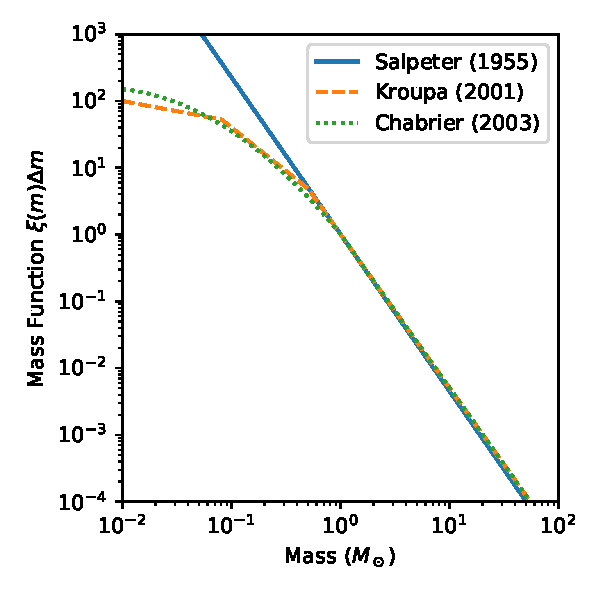
\includegraphics[width = 0.5\textwidth]{figs/imf.pdf}
\caption{Initial mass functions by \cite{salpeter55}, \cite{kroupa01}, and \cite{chabrier03}.}
\label{fig:imf}
\end{figure}

\subsubsection{Stellar Nucleosynthesis Yields}

Stellar nucleosynthesis yields are another important input in GCE models. The chemical enrichment in galaxies is due to the chemical elements produced in stars and recycled back to the ISM when they die. The nucleosynthesis yield of a star depends on its mass.

For stars with $M<0.8\msun$, their lifetime exceeds the Hubble time. Therefore, they can only lock up gas and have limited contribution to GCE.

Intermediate-mass stars with $M\lesssim 8 \msun$ form some $\alpha$ elements (e.g. C and O) and are the main site for the slow neutron capture process ($s$-process) which produces heavy elements (e.g. Ba, Sr, Y). These stars die as a C-O white dwarf (WD) and leave behind a planetary nebula. The material in the C-O WD is locked up, while the material in the planetary nebula is recycled back into the ISM. In binary systems, intermediate stars can die as Type Ia SNe (SNe-Ia). SNe-Ia significantly contribute to the iron-peak elements. However, since they require two fully evolved stars, they can only contribute on a large timescale.

Massive stars with $8\msun<M<10\msun$ likely explode as electron-capture supernovae (ECSNe). However, the detailed mechanism behind ECSNe is still largely unknown. Massive stars with $M>10\msun$ are expected to explode as core-collapse supernovae (CCSNe). Massive stars with $8\msun<M\lesssim 25\msun$ mainly produce alpha elements, iron-peak elements, and part of the slow neutron capture process (\textit{s}-process) elements. It is also possible that CCSNe can host rapid neutron process (\textit{r}-process) and can contribute to the production of proton-nuclei (\textit{p}-nuclei).

\subsubsection{Gas Flows}

When building a realistic model of a galaxy, it is important to consider the inflow and outflow of gas. GCE models that do not take into account these processes are known as closed-box models. The main effect of gas inflow and outflow in GCE models is to change the metallicity of the galaxy.

Gas inflows are generally considered to be either gas accretions or radial gas flows. Typically, gas is assumed to flow in from the metal-poor halo, with a primordial composition, as the material in the halo has not been processed through the GCE. Gas outflows also change the metallicity of the galaxy by reducing the amount of gas available for star formation. Galactic gas outflows are primarily caused by SNe, which accelerate the gas and transport it away from the galaxy.

\subsection{Galactic Chemical Evolution Models}

\subsubsection{One-Zone GCE Model}

The one-zone model is one of the simplest GCE models. In this model, the materials released from stars are immediately recycled back into the galaxy. The evolution of an element $X_i$ as a function of time can be written as:

\begin{equation}
\frac{d(X_if_g)}{dt} = E_{SW} + E_{CCSN} + E_{SNIa} + E_{NSM} - X_i\psi + X_{i, in}R_{in} - X_iR_{out},
\end{equation}

where $f_g$ is the fraction of mass that is in gas form, and $E_{SW}$, $E_{CCSN}$, $E_{SNIa}$, and $E_{NSM}$ are stellar ejections in the form of stellar wind, CCSNe, SNe-Ia, and neutron star mergers, respectively. $X_{i, in}$ is the mass fraction of the element in the inflow gas, and $R_{in}$ is the inflow rate, while $R_{out}$ is the outflow rate.

Although the one-zone model is a good first-order approximation, it cannot track the heterogeneity evolution of the galaxy due to the instantaneous mixing assumption. However, it is a simple and self-consistent way to track the evolution of all the elements.

\subsubsection{Chemodynamical Models}

In contrast to one-zone models, chemodynamical models do not assume that stellar feedback is instantaneously available throughout the entire galaxy. Instead, each nucleosynthesis event is modeled using star particles, and feedback from these particles is mixed in the galaxy using a hydrodynamical prescription.

\subsubsection{Uncertainties and the Impact of Assumptions in GCE Models}

Because one-zone models are simple, they can be combined with a Markov Chain Monte Carlo (MCMC) code to study uncertainties and the impact of modeling assumptions in the GCE model. \cite{cote17} presented a simple galactic chemical evolution code, OMEGA, which, when combined with an MCMC calculation, reproduced the observed abundance evolution of O, Mg, Si, Ca, Ti, Cr, Mn, Ni, and Co in Sculptor, a dwarf spheroidal galaxy. The authors found the best set of parameters, along with their confidence levels. They concluded that chemical evolution results are primarily affected by the stellar nucleosynthesis yields used, rather than the complexity of the galaxy model itself. Therefore, simple one-zone models can sufficiently constrain GCE and validate stellar nucleosynthesis models.

\section{Stardust Grains}
\subsection{The origin of Stardust Grains}
Stardust grains are solid materials that form in the outflows of dying stars and subsequently mix into the interstellar medium. During the formation of the solar system, stardust grains were incorporated into meteorite parent bodies and can be found in primitive meteorites. Figure \ref{fig:stardust_origin} shows a schematic of the history of stardust grains. Stardust grains contain the nucleosynthesis signature of their parent star, and we can make high-precision measurements of their isotopic composition. Therefore, they are useful in constraining galactic chemical evolution (GCE) and stellar nucleosynthesis models.

\begin{figure}[htbp]
\centering
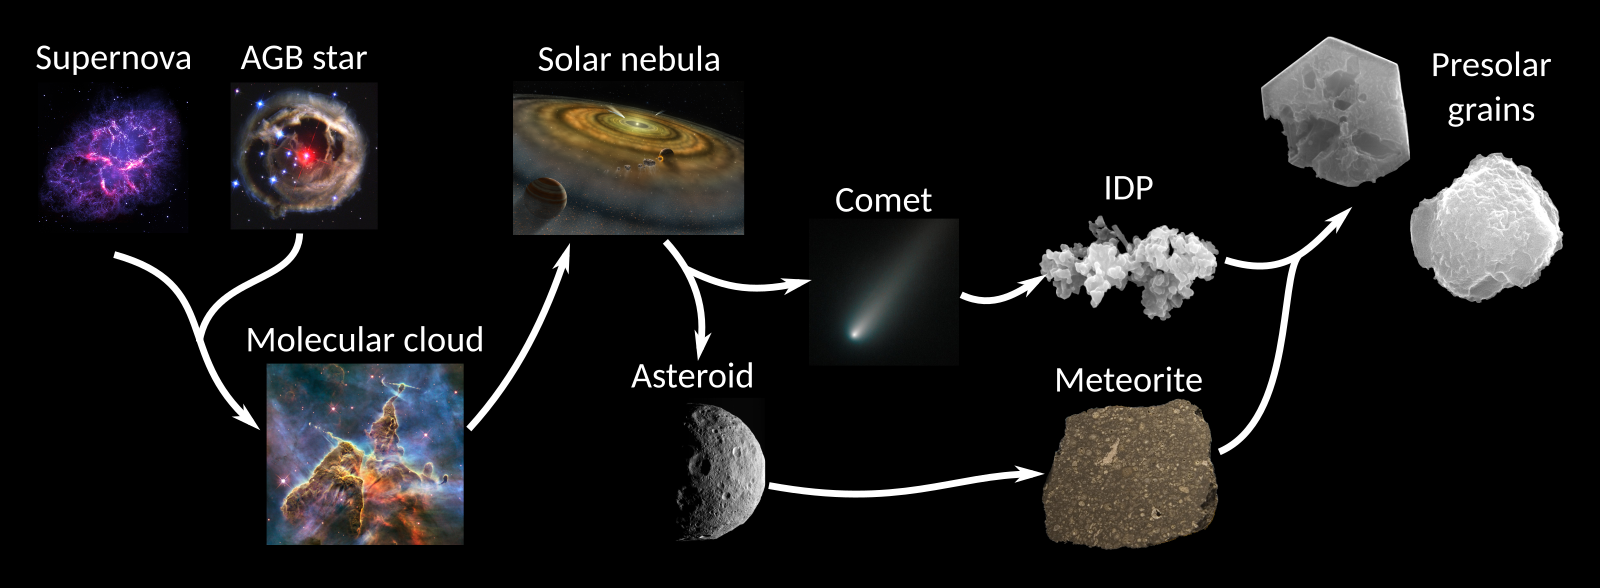
\includegraphics[width = 0.9\textwidth]{figs/presolar_grains_origin_1600.png}
\caption{Schematic of the origin of stardust grains}
\label{fig:stardust_origin}
\end{figure}

\subsection{Types of Stardust Grains}
One of the best-studied stardust grains is silicon carbide (SiC) grains (figure \ref{fig:sic_pic}). The SiC grains have sizes up to several micrometers and can be separated from meteorites and studied individually in the laboratory. Other types of stardust grains include nanodiamonds and graphite grains. Nanodiamonds are the most abundant type of stardust grains. However, these particles are only several nanometers in diameter. Due to their relatively small sizes, they are not able to be studied directly in the laboratory. Graphite grains can also be separated from meteorites. They also occur in large sizes. However, they often show contamination with solar system material due to the nature of graphite.

\subsection{Silicon Carbide Grains}
Measurements of the SiC grains can be particularly useful in constraining stellar nucleosynthesis and GCE models. These grains are generally analyzed by mass spectrometry for their isotopic composition. The isotopic measurement is usually expressed as ratios with respect to the most abundant isotope in $\delta$-notation,
\begin{equation}
\delta(\frac{^iX}{^jX}) = \delta^i X_j = \left[ \frac{\left( \frac{^iX}{^jX}\right)_{sample}}{\left(\frac{^iX}{^jX}\right)_{\odot}} - 1\right] \times 1000\ (\permil)
\end{equation}

\begin{figure}[htbp]
\centering
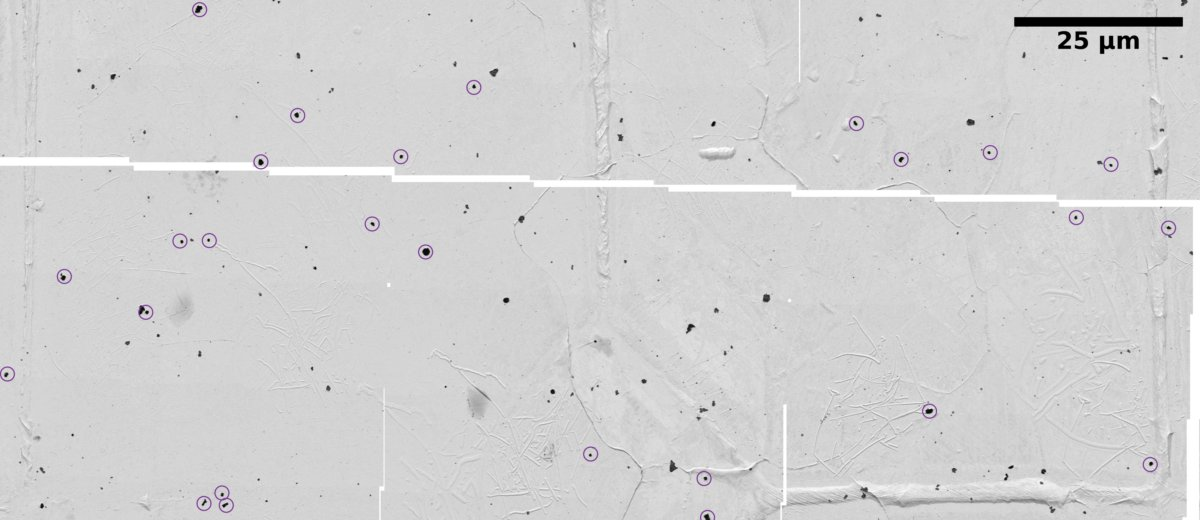
\includegraphics[width= 0.9\textwidth]{figs/sem_mount-s.jpg}
\caption{A section of a presolar grain. Identified SiC grains are circled in purple.}
\label{fig:sic_pic}
\end{figure}

\subsubsection{Classification of SiC Grains}
Based on its C, N, and Si isotopic composition, SiC grains can be divided into different populations (figure \ref{fig:sic}). Most of the SiC grains belong to the so-called mainstream (M) group. The mainstream grains are believed to come from $1.5-3\msun$ AGB stars with roughly solar metallicity. Another important type of presolar SiC grains is the so-called X grains which are characterized by their overabundance in \iso{28}{Si}, \iso{12}{C}, and \iso{15}{N} as shown in figure \ref{fig:sic}. The X grains are believed to form in the ejecta of core-collapse supernovae. Other types of SiC grains of likely SNe origin are grains of type AB, C, X, and nova. 

\begin{figure}
     \centering
     \begin{subfigure}[b]{0.45\textwidth}
         \centering
         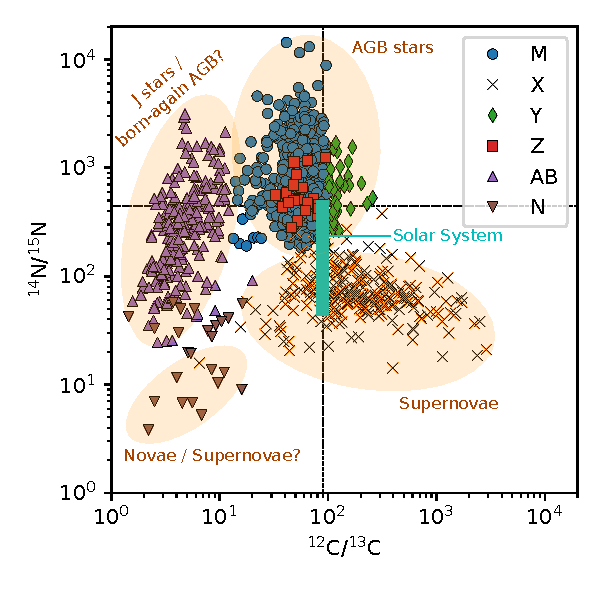
\includegraphics[width=\textwidth]{figs/sic_n_c_all.pdf}
        %  \caption{}
     \end{subfigure}
     \begin{subfigure}[b]{0.45\textwidth}
         \centering
         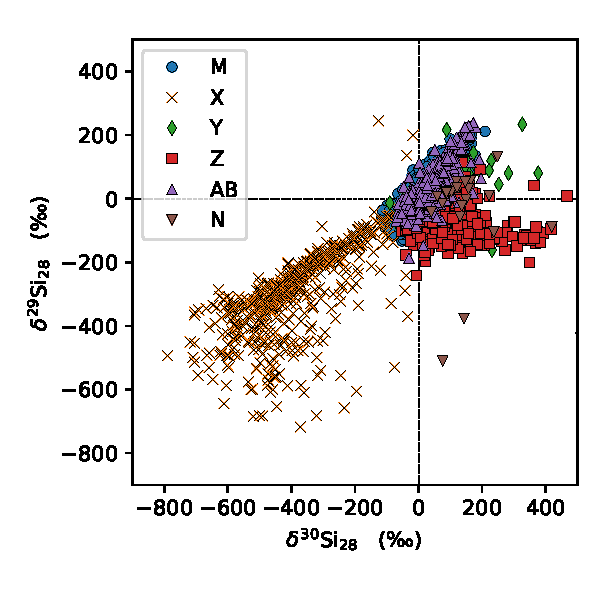
\includegraphics[width=\textwidth]{figs/sic_si_3iso_all.pdf}
        %  \caption{}
     \end{subfigure}
     \caption{(Left) Nitrogen and carbon isotopic composition of analyzed SiC grains. The data is represented as the ratio with respect to the most abundant isotope of nitrogen and carbon. (Right) Silicon isotopic composition of SiC grains. The data is represented in $\delta$-notation. The data taken from \cite{stephan_20}.}
     \label{fig:sic}
\end{figure}

\section{Silicon Isotopes in Mainstream Grains and GCE}
The silicon isotopic composition of the mainstream grains is characterized by enrichment in heavy silicon isotopes of up to $200\permil$ relative to the solar system composition. Moreover, in the so-called silicon three-isotope plot, the mainstream grains data shows a correlation between their \iso{29}{Si}/\iso{28}{Si} and \iso{30}{Si}/\iso{28}{Si} ratios. In particular, they fall along the so-called Si mainstream line $\del{29}{28}{Si} = 1.37 \times \del{30}{28}{Si} -20$ (\citealt{Zinner2007}). Although the mainstream grains come from AGB stars, the silicon isotopic ratios of mainstream grains cannot be explained by nucleosynthesis in their parent stars (\citealt{Lugaro1999}). Instead, the Si mainstream line represents the GCE of silicon isotopes. However, the current GCE models fail to explain the silicon isotopic abundance measured in the mainstream grains. There are mainly three problems:
\begin{enumerate}
    \item The scatter in the Si isotopic compositions of the parent stars shown by the mainstream grains measurements;
    \item Most of the mainstream grains have higher than solar \iso{29}{Si}/\iso{28}{Si} and \iso{30}{Si}/\iso{28}{Si} ratios. In the GCE picture, the \iso{29}{Si}/\iso{28}{Si} and \iso{30}{Si}/\iso{28}{Si} ratios increase with metallicity which is a proxy for time;
    \item The slope of the Si mainstream line is larger than the prediction by the GCE models.
\end{enumerate}

\begin{figure}
    \centering
    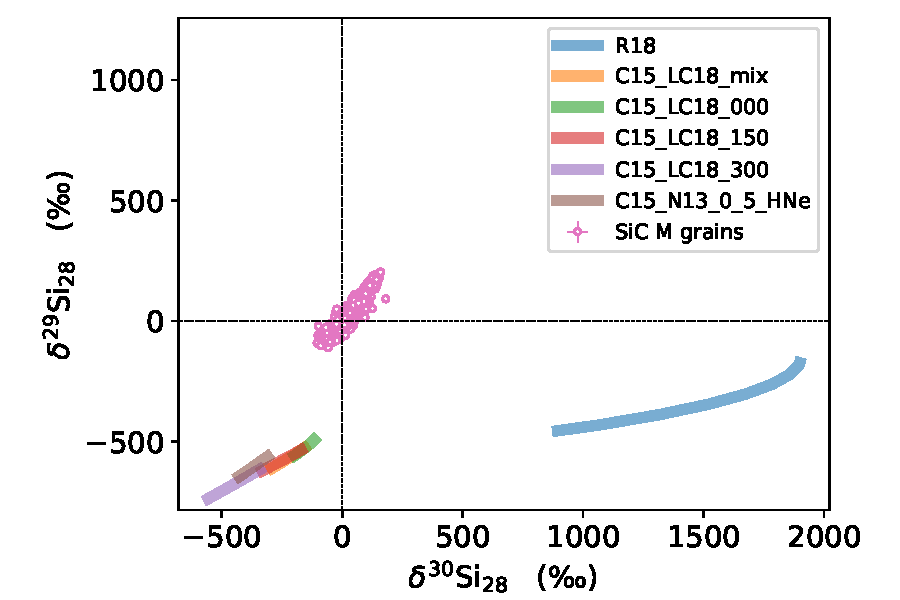
\includegraphics[width = 0.6\textwidth]{figs/gce_Si_isotope.pdf}
    \caption{Comparison between the GCE model and the mainstream grain data. GCE is simulated using OMEGA+ (\citealt{Cote_2018}) with different stellar yield sets available in the JINAPyCEE\protect\footnotemark  package.}
    \label{fig:gce_si}
\end{figure}

Different solutions have been proposed for the first two problems. \cite{Lugaro1999} explained the scatter using local heterogeneities in the regions from which the parent stars of the mainstream grains originally formed due to the stochastic nature of the admixture of the contributions from supernovae of varying mass and type. \cite{Clayton1997} addressed the second problem by considering star migration. The mainstream grains might be originated from stars that were born in central, more metal-rich regions of the galaxy and moved to the molecular cloud from which the solar system is formed. 
\footnotetext{https://github.com/becot85/JINAPyCEE}

On the other hand, the discrepancy between the slope of the Si mainstream line and the slope predicted by GCE models remains largely unexplained. There have been indications that the nuclear uncertainties in stellar nucleosynthesis calculations might be able to explain the problem (\citealt{Timmes_1996}; \citealt{Hoppe_2009}). In particular, \cite{Hoppe_2009} has shown that increasing the rate of \iso{26}{Mg}$(\alpha, n)$\iso{29}{Mg} by a factor of 3 will lead to an increase in the \iso{29}{Si}/\iso{28}{Si} by a factor of 1.8 with the \iso{30}{Si}/\iso{28}{Si} ratios largely unchanged. Such an increase is able to explain the Si isotopic abundance measured in a grain which is believed to come from a CCSN (\citealt{Hoppe_2009}). In our work, we aim to quantify the effect of nuclear uncertainties on the GCE of Si isotopes in a more physical way using a Monte Carlo method. The steps in our work can be summarized as follows:
\begin{enumerate}
    \item Identify the stars that are responsible for the production of silicons in the galaxy;
    \item Identify the main Si-production regions in those stars and the relevant reactions for Si production;
    \item Calculate the nucleosynthesis in the relevant regions and the resulting stellar nucleosynthesis yield with varying reaction rates;
    \item Calculate the GCE of the Si isotopes using the modified stellar yields.
\end{enumerate}

Through these steps, we aim to answer the following question: can nuclear uncertainties explain the model-data discrepancy of the Si isotopic ratios observed in the mainstream grain? In chapter \ref{method}, we discuss the numerical models we used for nucleosynthesis and GCE calculations and the pipeline we developed connecting the two calculations, as well as the Monte Carlo setup. In chapter \ref{result}, we show results from the nucleosynthesis and GCE calculations and compare them with presolar grains data. In chapter \ref{conclusion}, we summarize the main results and discuss the implications and future works.



\chapter{Method} \label{method}


\section{Nucleosynthesis Simulation} \label{nucleosynthesis}
In our work, the nucleosynthesis simulations are calculated using the single-zone frame PPN of the NuGrid\footnote{https://nugrid.github.io} post-processing code. In the post-processing approach, a small nuclear network, large enough to account for the nuclear energy generation, is used for the stellar evolution simulations. The stellar evolution data for all zones at all time steps are then post-processed using a full nuclear network for nucleosynthesis calculation. This can be done either at one Lagrangian coordinate (with the single-zone code PPN) or for an entire star (with the multizone code MPPNP). In the case of the single-zone code PPN, changes in temperature $T$ and density $\rho$ with time at the chosen zone (the so-called trajectory) have to be provided. The initial condition for the network calculation will be the initial isotopic abundance. In order to get a consistent result, the post-processing network needs to adopt the same nuclear physics for the reactions used in the stellar evolution calculation. 

For our work, the stellar structure evolution data (trajectory) is obtained from the NuGrid stellar evolution models (\citealt{Pignatari_2016}; \citealt{Ritter_2018}). In the NuGrid models, the stellar evolution calculations were performed using the MESA stellar evolution code (\citealt{Paxton_2011}). For the CCSN explosions, the NuGrid models use a semi-analytic approach with the shock launched from the protoneutron stars based on a mass cut derived from \cite{Fryer_2012}. In our work, we use the delayed-convection explosions models for CCSNe explosions. 

% \section{Stellar Nucleosynthesis Yield Integration} \label{yield}
% In order to get the stellar nucleosynthesis yield 

\section{Galactic Chemical Evolution Simulations} \label{gce}
In our work, we use the 2-zone semi-analytic GCE model OMEGA+ (\citealt{Cote_2018}). OMEGA+ consists of a star-forming region (the galaxy) surrounded by a hot gas reservoir filling the dark matter halo of the host galaxy (the circumgalactic medium CGM). The star-forming region is assumed to contain the stellar population in the galaxy and is simulated using the open-boxed one-zone GCE model OMEGA (One-zone Model for the Evolution of GAlaxies; \citealt{cote17}). The OMEGA code calculates the chemical mixture of the ISM as a function of time using a given input star formation history. The calculation takes into account the contribution of multiple stellar populations, as well as the effect of galactic inflows and outflows. The role of OMEGA+ is to interact with OMEGA at each time step to control the rate of inflow, outflow, and star formation. 

The time evolution of the mass of the gas in the star-forming region $M_{gas}$ is defined by
\begin{align}
    \dot{M}_{gas} &= \dot{M}_{g, in}\ +\ \dot{M}_{ej}\ -\ \dot{M}_{*}\ -\ \dot{M}_{g, out},
\end{align}
where the terms on the right-hand side are the galactic inflow rate $\dot{M}_{g, in}$, mass-loss rate of all stars $\dot{M}_{ej}$, the star formation rate $\dot{M}_{*}$, and the galactic outflow rate $\dot{M}_{g, out}$ respectively.

The time evolution of the mass of circumgalactic medium $M_{CGM}$ is defined by
\begin{align}
     \dot{M}_{CGM} &= \dot{M}_{CGM, in}\ +\ \dot{M}_{g, out}\ -\ \dot{M}_{g, in}\ -\ \dot{M}_{CGM, out},
\end{align}
where $\dot{M}_{CGM, in}$ is the circumgalactic inflow rate and $\dot{M}_{CGM, out}$ is the circumgalactic outflow rate. 

\begin{figure}
    \centering
    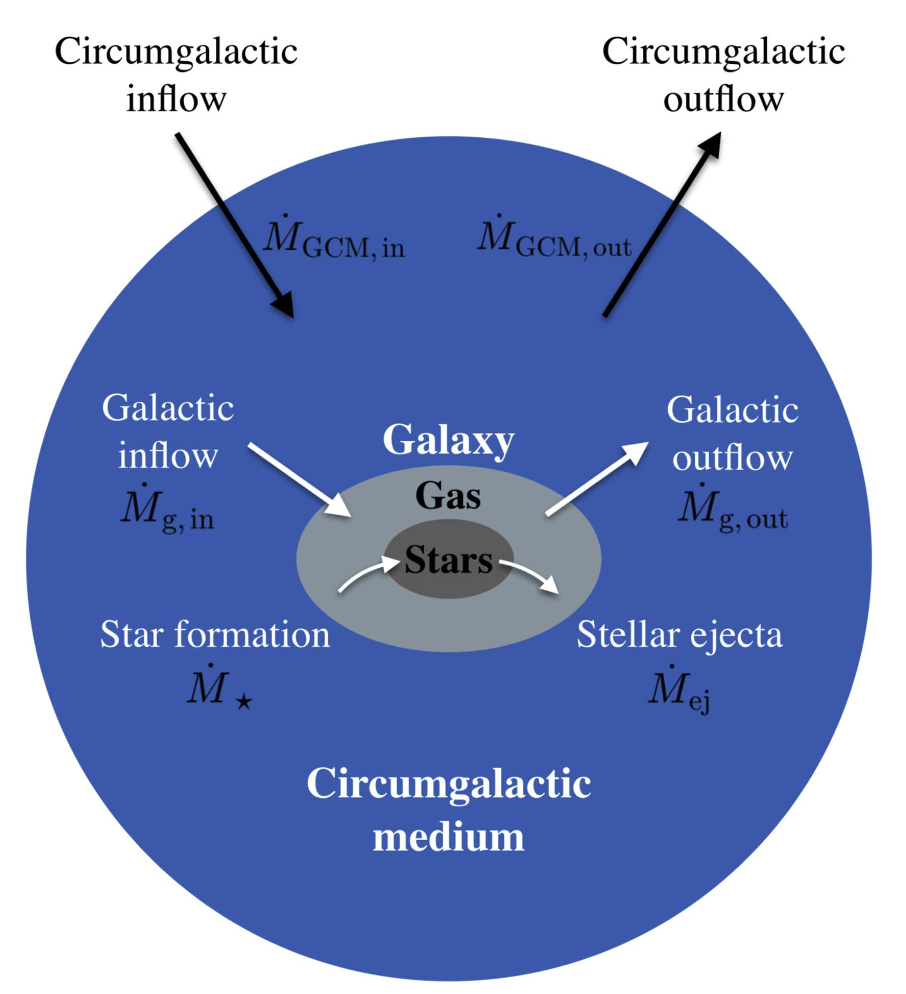
\includegraphics[width = 0.5\textwidth]{figs\omega.pdf}
    \caption{Caption}
    \label{fig:omega}
\end{figure}

The galactic inflow rate is defined by 
\begin{align}
    \dot{M}_{g, in} = \frac{M_{CGM}}{\tau_{inflow}},
\end{align}
where $\tau_{inflow}$ is the inflow timescale. 

The circumgalactic inflow rate is defined by 
\begin{align}
    \dot{M}_{CGM, in} = \dot{M}_{DM} \left( \frac{\Omega_{M, 0}}{\Omega_{b, 0}} - 1\right)^{-1},
\end{align}
where $\dot{M}_{DM}$ is the growth rate of the dark matter mass and $\Omega_{b, 0}/\Omega_{M, 0}$ is the universal baryonic fraction.


The star formation rate is defined by 
\begin{align}
    \dot{M}_{*} = f_{*}M_{gas},
\end{align}
where $f_*$ is the star formation efficiency. 

The galactic outflow rate is defined using the mass-loading factor $\eta_{gal}$, 
\begin{align}
    \eta_{gal} = \frac{\dot{M}_{g, out}}{\dot{M}_{*}}.
\end{align}

Similarly, the circumgalacic outflow rate can be defined using the mass-loading factor $\eta_{CGM}$, 
\begin{align}
    \eta_{CGM} = \frac{\dot{M}_{CGM, out}}{\dot{M}_{*}},
\end{align}
and is assumed to be proportional to the galactic outflow rate through the parameter $f_{\eta}$, 
\begin{align}
    \dot{M}_{CGM, out} = f_\eta \eta_{gal} \dot{M}_{*}.
\end{align}

The mass-loss rate of all stars $\dot{M}_{ej}$ is given by the stellar nucleosynthesis yields. 


\section{Pipeline}
To investigate the impact of nuclear uncertainties on the GCE of silicon isotopes, we developed a pipeline connecting stellar nucleosynthesis simulation with GCE simulation. 

There are three main parts in our pipeline: stellar nucleosynthesis simulation (\ref{nucleosynthesis}), stellar nucleosynthesis yield calculation, and GCE simulation (\ref{gce}). The general workflow is shown in figure \ref{fig:workflow}
\begin{figure}
    \centering
    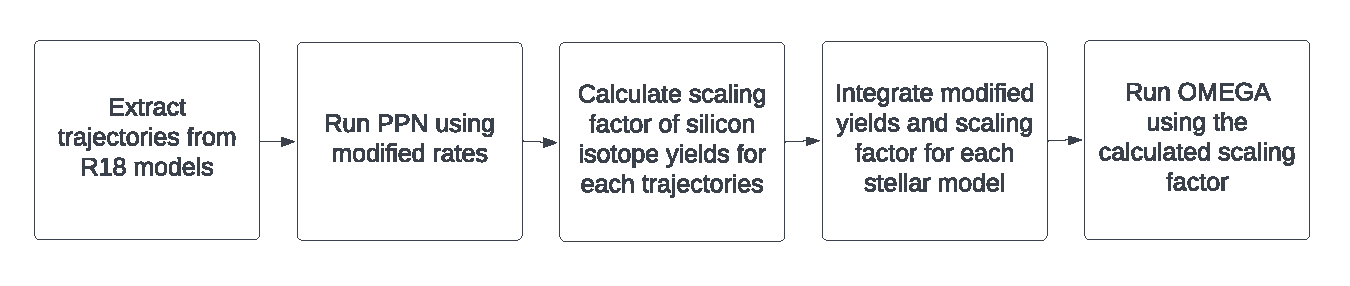
\includegraphics{flowchart.pdf}
    \caption{Caption}
    \label{fig:workflow}
\end{figure}

In order to 

\section{Monte Carlos Setup}

\chapter{Result} \label{result}

\section{Stellar Population Responsible for Silicon Production in the Galaxy}
\section{Main Silicon Production Regions in Massive Stars}

\section{Comparison with SiC type C Grains}


\section{Stellar Nucleosynthesis Yields}

\section{Galactic Chemical Evolution of Silicon Isotopes}

\section{Comparison with SiC Mainstream Grains}

\chapter{Conclusion} \label{conclusion}


\singlespacing
\bibliography{ref}

\end{document}
